% !TEX TS-program = xelatex
\documentclass[aspectratio=169]{beamer}

% --- THEME & LAYOUT ---
\usetheme[numbering=fraction,progressbar=head]{metropolis}
\setbeamersize{text margin left=8mm,text margin right=8mm}

% --- CUSTOM FOOTER WITH TLP MARKING ---
\setbeamertemplate{frame footer}{\textbf{TLP:CLEAR} -- Information may be shared freely without restriction.}
\setbeamercolor{frame footer}{fg=cyber-accent}

\usepackage{amsmath}

% --- FONTS (XeLaTeX) ---
\usepackage{fontspec}
\setsansfont[
  Ligatures=TeX, Scale=1.02,
  BoldFont = {IBM Plex Sans Bold},
  ItalicFont = {IBM Plex Sans Italic}
]{IBM Plex Sans}
\setmonofont{IBM Plex Mono}

% --- ICONS ---
\usepackage{fontawesome5}

% --- COLORS (cyber palette) ---
\definecolor{cyber-bg}{HTML}{0B0F14}
\definecolor{cyber-ink}{HTML}{E6EEF5}
\definecolor{cyber-accent}{HTML}{217EAA}
\definecolor{cyber-mid}{HTML}{7D9CB7}
\definecolor{cyber-soft}{HTML}{8CA4AC}
\setbeamercolor{normal text}{fg=cyber-ink,bg=cyber-bg}
\setbeamercolor{frametitle}{fg=cyber-ink,bg=cyber-bg}
\setbeamercolor{progress bar}{fg=cyber-accent,bg=cyber-soft}
\setbeamercolor{alerted text}{fg=cyber-accent}

% --- LINKS ---
\hypersetup{colorlinks=true, linkcolor=cyber-accent, urlcolor=cyber-accent}

% --- CODE / BOXES ---
\usepackage{listings}
\lstset{
  basicstyle=\ttfamily\footnotesize,
  backgroundcolor=\color{black!5},
  frame=single, rulecolor=\color{cyber-soft},
  keywordstyle=\color{cyber-accent}\bfseries,
  commentstyle=\color{cyber-soft},
  showstringspaces=false
}
\usepackage[most]{tcolorbox}
\tcbset{colback=black!5!cyber-bg, colframe=cyber-soft, coltext=cyber-ink, boxsep=1mm, left=2mm, right=2mm}

% --- PDF TOOLS ---
\usepackage{pdfpages}

% --- GRAPHICS ---
\usepackage{graphicx}

% --- SPEAKER NOTES ---
\usepackage{pgfpages}
% \setbeameroption{hide notes}
% \setbeameroption{show notes}
% \setbeameroption{show only notes}

% --- SPACING IMPROVEMENTS ---
\setbeamertemplate{itemize/enumerate body begin}{\vspace{-0.5ex}}
\setbeamertemplate{itemize/enumerate subbody begin}{\vspace{-0.5ex}}

% --- TITLE INFO ---
\title{\faIcon{shield-alt}\; Range42 -- Progress \& Live Demo}
\subtitle{Open Cyber Range Platform for Collaborative Security Training}
\author{NC3 / Range42 Team}
\date{FIC Lille 2026}
\institute{\faServer\; Proxmox \quad \faCogs\; Ansible \quad \faProjectDiagram\; Orchestration \quad \faBinoculars\; Telemetry}

\begin{document}

% === TITLE ===
\begin{frame}[plain,noframenumbering]
  \titlepage
  \note[item]{Goal: 20-minute overview of Range42's progress since 2025 with a live demo of the deployer UI.}
  \note[item]{Audience: cybersecurity professionals, government, European ecosystem partners.}
\end{frame}

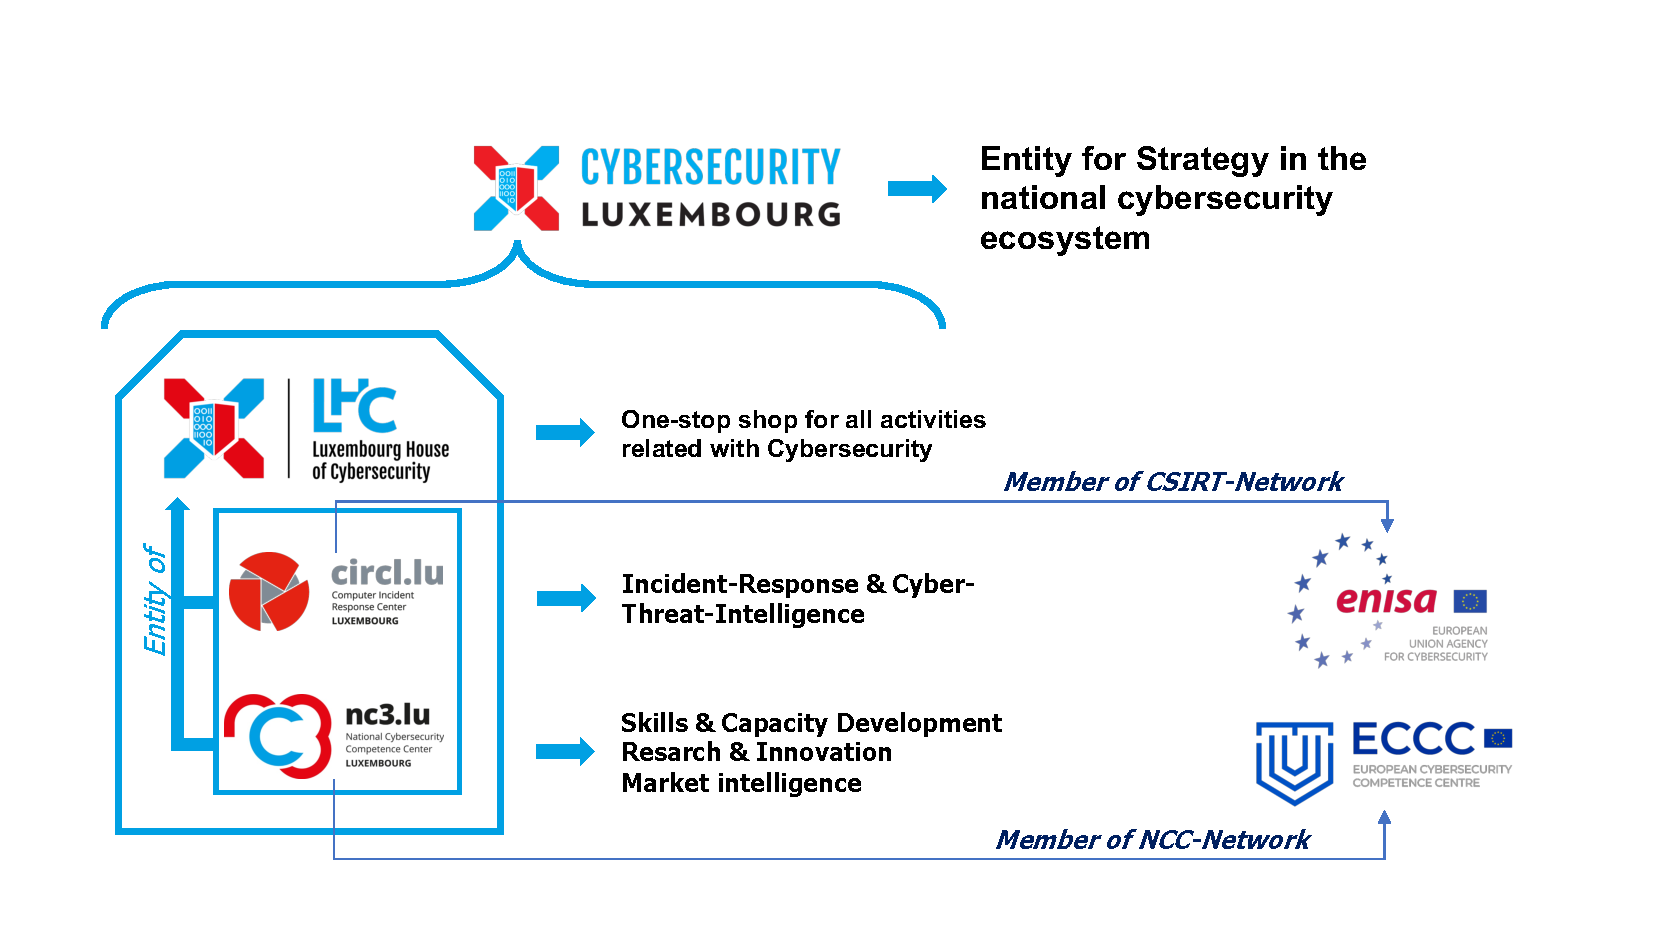
\includepdf[pages={1-2}]{../../pdf_slides/LHC_NC3.pdf}

% === PUBLIC MONEY PUBLIC CODE ===
\begin{frame}{Public Money, Public Code. Let's go all the way, shall we?}
  \begin{columns}[T]
    \column{0.65\textwidth}
    \textbf{Team \& Funding}
    \begin{itemize}
      \item Core team of 3 -- InfoSec \& DevOps engineers
      \item Collaboration model with NC3 \& ecosystem partners
      \item Public grant for cyber training infrastructure
      \item FOSS model: no licensing \textcolor{green}{\faMoneyBill}, transparent development
    \end{itemize}

    \column{0.3\textwidth}
    \vspace{2mm}
    \begin{figure}
      \centering
      
\includegraphics[width=\textwidth]{../../images/logos/FSFE_Public_Money_Public_Code_logo.pdf}
    \end{figure}
  \end{columns}
  \note[item]{Emphasize public funding = public ownership = public benefit.}
\end{frame}

% === AGENDA ===
\begin{frame}{Agenda}
  \begin{enumerate}
    \item What Range42 is \& why it matters
    \item Progress since 2025: what's new
    \item Architecture overview
    \item \alert{Live demo}: the Deployer UI in action
    \item What's possible today vs.\ what's coming
    \item Development roadmap: 6 strategic axes
    \item How to get involved
  \end{enumerate}
  \note[item]{Highlight the demo as the centerpiece of this talk.}
\end{frame}

% === WHAT IS RANGE42 ===
\begin{frame}{What is Range42?}
  \begin{itemize}
    \item \textbf{Open cyber range platform} for offensive, defensive, and hybrid training
    \item \textbf{Reproducible Infrastructure-as-Code}: Proxmox, Ansible, Docker
    \item \textbf{Flexible \& extensible}: supports CVE labs, misconfigurations, forensics, malware analysis
  \end{itemize}
  \begin{tcolorbox}
    \faInfoCircle\; Built to simulate \emph{real-world incidents} safely, with isolation, snapshots, and telemetry.
  \end{tcolorbox}
  \note[item]{Anchor on "safe realism" and extensibility.}
\end{frame}

% === PROGRESS SINCE 2025 ===
\section{Progress Since 2025}

\begin{frame}{Progress Since 2025 \; \faChartLine}
  \textbf{By the Numbers}
  \begin{itemize}
    \item \alert{520+ total commits} across 14 repositories (up from 400+)
    \item Backend API: 156 commits -- \textbf{major refactor} (86 routes $\rightarrow$ 10 modules)
    \item Deployer UI: 74 commits -- from prototype to \textbf{functional tool}
    \item Proxmox controller: 112 commits -- cloud-init, VM templates, storage
  \end{itemize}
  \vspace{1mm}
  \textbf{Key Milestones}
  \begin{itemize}
    \item \alert{Docker deployment} for the backend API
    \item \alert{Real-time VM status} via WebSocket on the canvas
    \item \alert{Comprehensive test suite} and Sphinx documentation
    \item \alert{CyCon 2026 paper submitted} -- academic publication
  \end{itemize}
  \note[item]{Concrete, measurable progress. This is not vaporware.}
\end{frame}

% === CURRENT ACHIEVEMENTS ===
\begin{frame}{Current Achievements \; \faCheckCircle}
  \textbf{What's Working Today}
  \begin{itemize}
    \item \alert{$\sim$100 CVEs \& misconfigurations identified}, $\sim$20 deployable scenarios
    \item \textbf{Automated provisioning} on Proxmox with networking, VPN, firewalling
    \item \textbf{Visual lab designer} with drag-and-drop infrastructure composition
    \item \textbf{Integrated monitoring} via Wazuh for telemetry and alerting
    \item \textbf{14 repositories} managing automation, content, and tooling
  \end{itemize}
  \vspace{2mm}
  \begin{tcolorbox}
    \faLightbulb\; \textbf{Key Milestone}: Backend is production-ready. The visual designer is now functional and actively used.
  \end{tcolorbox}
  \note[item]{Emphasize: both backend AND frontend are operational now.}
\end{frame}

% === COMPETITIVE LANDSCAPE ===
\begin{frame}[shrink=5]{Range42 vs.\ Other Cyber Ranges}
  \begin{table}
    \tiny\color{cyber-ink}
    \begin{tabular}{l|cccc}
      \textbf{Feature} & \textbf{Range42} & \textbf{Commercial SaaS} & \textbf{Cloud Native} & \textbf{Traditional} \\
      \hline
      \alert{Open Architecture} & \checkmark & \texttimes & \texttimes & \texttimes \\
      \alert{IaC/GitOps} & \checkmark & \textasciitilde & \checkmark & \texttimes \\
      Private Deployment & \checkmark & \texttimes & \textasciitilde & \checkmark \\
      Cost Control & \checkmark & \texttimes & \textasciitilde & \checkmark \\
      Full Data Custody & \checkmark & \texttimes & \texttimes & \checkmark \\
      API Orchestration & \checkmark & \checkmark & \checkmark & \texttimes \\
      Rapid Reset/Snapshots & \checkmark & \checkmark & \textasciitilde & \textasciitilde \\
      Custom Scenarios & \checkmark & \texttimes & \textasciitilde & \checkmark \\
      \alert{Visual Lab Designer} & \checkmark & \checkmark & \texttimes & \texttimes \\
    \end{tabular}
  \end{table}
  \vspace{1mm}
  \begin{tcolorbox}
    \faLightbulb\; \textbf{Range42's Edge}: Full control, reproducibility, and cost-effectiveness without vendor lock-in.
  \end{tcolorbox}
  \note[item]{Added visual lab designer row -- new differentiator since 2025.}
\end{frame}

% === ARCHITECTURE ===
\begin{frame}[squeeze]{Architecture at a Glance}
  \begin{itemize}
    \item \textbf{Hypervisor layer}: Proxmox VMs/LXCs; snapshots; network segments
    \item \textbf{Automation layer}: Ansible roles orchestrate lifecycle, network, firewall, images
    \item \textbf{Control plane}: Backend API (FastAPI) with Docker deployment; WebSocket for live status
    \item \textbf{UX layer}: Deployer UI (visual designer), Exercise Management Platform (in development)
    \item \textbf{Observability}: Wazuh for logs/alerts; structured telemetry
  \end{itemize}
  \note[item]{Highlight WebSocket and Docker as new additions to the architecture.}
\end{frame}

\begin{frame}[shrink=8]{Architecture: Logical Components $\rightarrow$ Repository Mapping}
  \begin{figure}
    \centering
    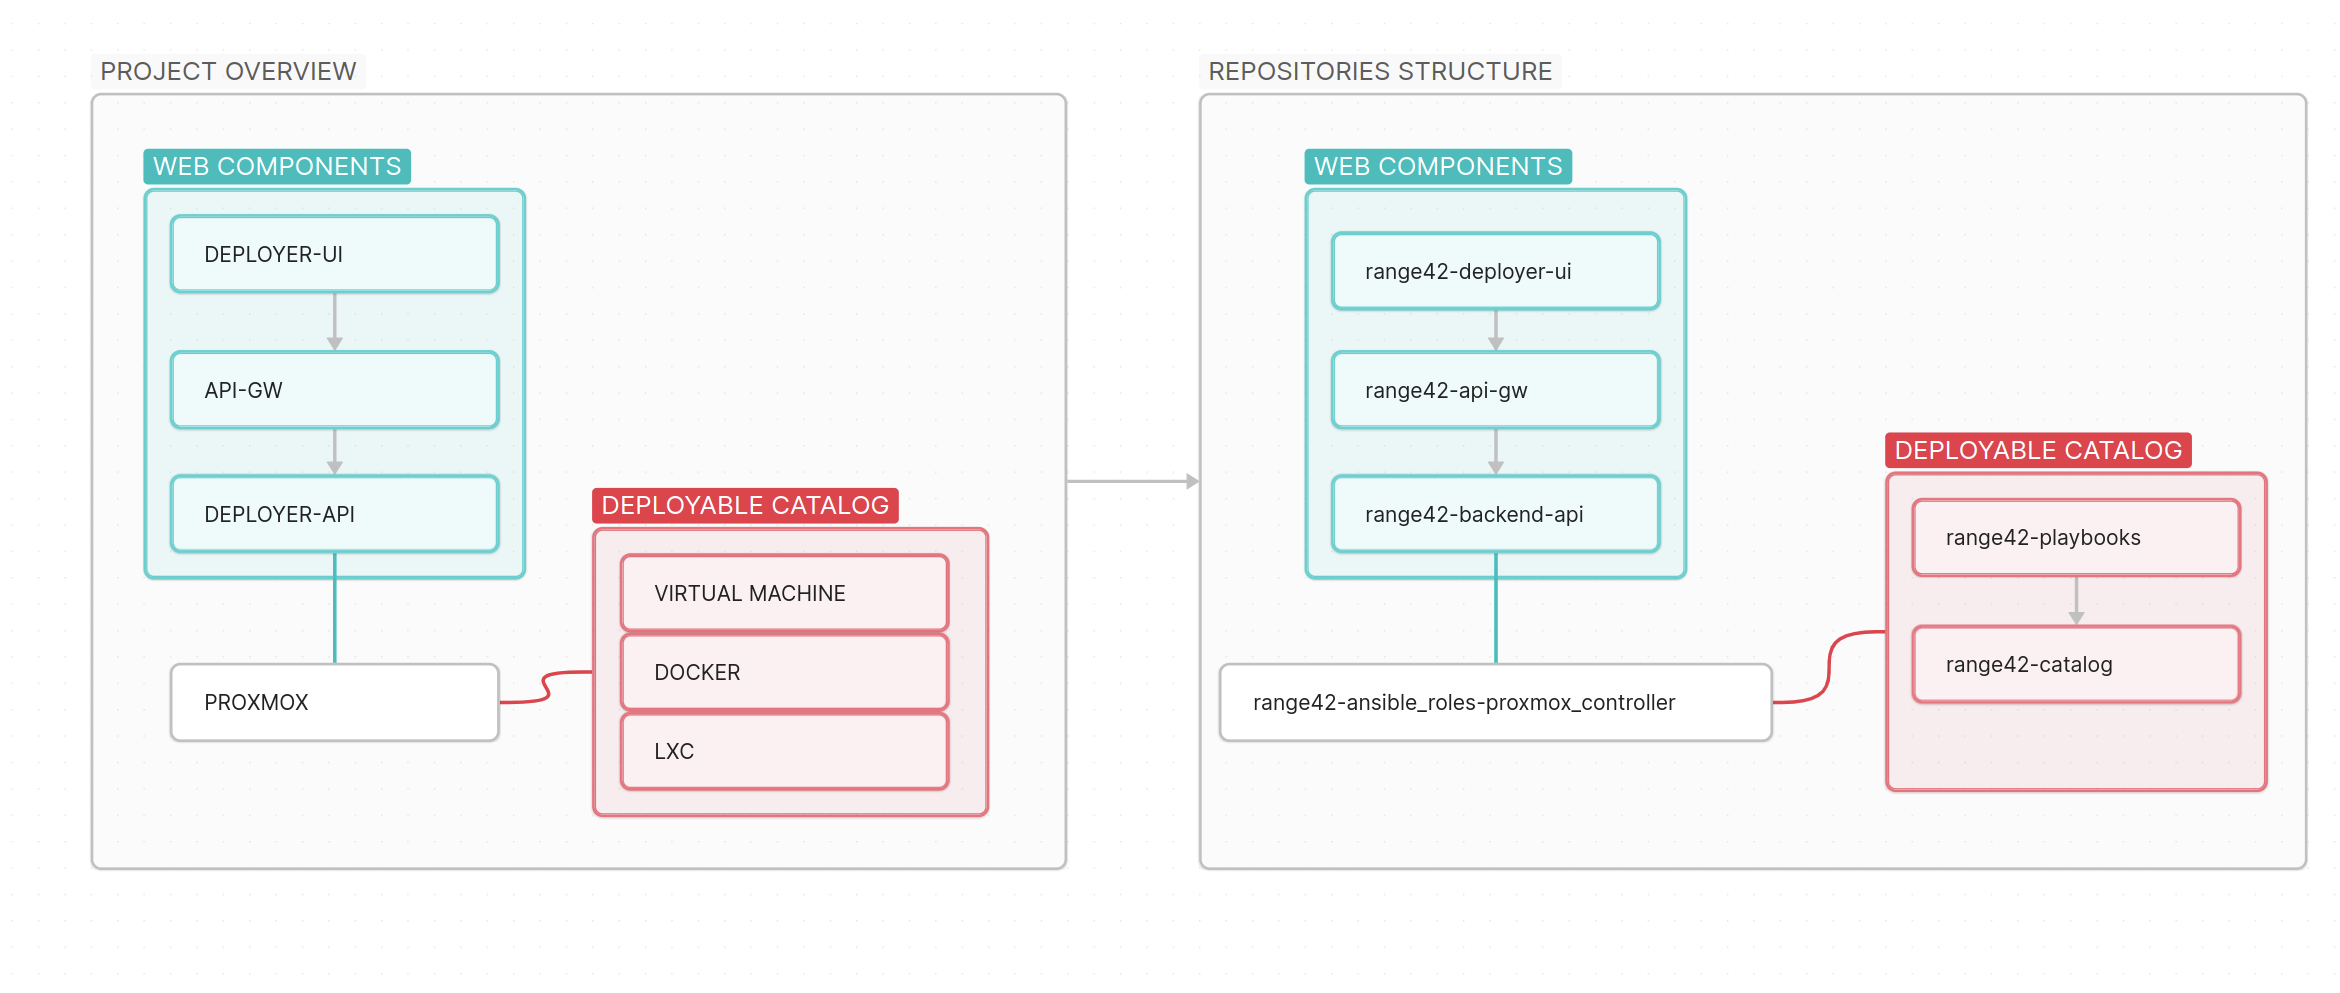
\includegraphics[width=0.95\textwidth]{../../images/diagrams/architecture.png}
  \end{figure}
  \vspace{-3mm}
  \begin{tcolorbox}
    \faInfoCircle\; \textbf{Left}: Logical architecture flow. \textbf{Right}: Actual GitHub repository structure.
  \end{tcolorbox}
  \note[item]{Left side shows logical architecture; right side shows actual GitHub repos.}
\end{frame}

% === DEPLOYER UI DEMO ===
\section{Live Demo: Deployer UI}

\begin{frame}{Deployer UI: Visual Lab Designer \; \faDrawPolygon}
  \begin{columns}[T]
    \column{0.48\textwidth}
    \textbf{\faEdit\; Design}
    \begin{itemize}
      \item Drag-and-drop VMs, LXC, networks, routers, firewalls
      \item Configure CPU, memory, disk, ISO per node
      \item Proxmox template selection with auto-fill
      \item Connect nodes to define topology
    \end{itemize}

    \column{0.48\textwidth}
    \textbf{\faPlay\; Deploy}
    \begin{itemize}
      \item Pre-deploy reconciliation and validation
      \item Ordered: networks $\rightarrow$ routers $\rightarrow$ VMs $\rightarrow$ config $\rightarrow$ start
      \item Real-time status via WebSocket
      \item Start, stop, restart, delete from the UI
    \end{itemize}
  \end{columns}
  \note[item]{Set up context before switching to the live demo.}
\end{frame}

\begin{frame}{Live Demo \; \faPlay}
  \begin{center}
    {\Large \faDesktop\quad Switch to live demo}\\[8mm]
    \textbf{Demo Flow}\\[4mm]
    \begin{enumerate}
      \item Create a new project on the canvas
      \item Add VMs, networks, and a router
      \item Configure VM templates and resources
      \item Deploy to Proxmox
      \item Watch real-time status updates
      \item Control VMs from the UI (start/stop)
    \end{enumerate}
  \end{center}
  \note[item]{This is the placeholder slide -- switch to the actual deployer UI here.}
  \note[item]{Keep demo under 5 minutes. Focus on the wow factor: design $\rightarrow$ deploy $\rightarrow$ live.}
\end{frame}

% === BACKEND API MATURITY ===
\begin{frame}{Backend API: Production-Ready \; \faCogs}
  \begin{columns}[T]
    \column{0.48\textwidth}
    \textbf{Major Refactoring}
    \begin{itemize}
      \item 86 route files $\rightarrow$ \textbf{10 domain modules}
      \item 52 schema files $\rightarrow$ grouped modules
      \item Application factory pattern
      \item Structured logging throughout
      \item Centralized secret management
    \end{itemize}

    \column{0.48\textwidth}
    \textbf{New Capabilities}
    \begin{itemize}
      \item \alert{Docker deployment} (compose)
      \item \alert{WebSocket API} for live status
      \item \alert{Test suite}: unit + integration
      \item \alert{Sphinx documentation}
    \end{itemize}
  \end{columns}
  \note[item]{Backend went from prototype-quality to production-grade.}
\end{frame}

% === TODAY VS FUTURE ===
\section{Today \& Tomorrow}

\begin{frame}{Today vs.\ Tomorrow}
  \begin{columns}[T]
    \column{0.48\textwidth}
    {\textbf{\faCheckCircle\; Operational Today}}
    \begin{itemize}
      \item Full Proxmox automation (VMs, LXC, network, firewall, VPN)
      \item Visual lab designer with drag-and-drop
      \item Real-time VM status via WebSocket
      \item Template provisioning + reconciliation
      \item Docker-based API deployment
      \item Wazuh monitoring integration
    \end{itemize}

    \column{0.48\textwidth}
    {\textbf{\faRocket\; Coming Next}}
    \begin{itemize}
      \item Exercise Management Platform (scoring \& reporting)
      \item LLM-assisted scenario generation
      \item Multi-subnet enterprise topologies
      \item Declarative Live State Engine
      \item ICS / IoT training scenarios
      \item Federated catalog exchange
    \end{itemize}
  \end{columns}
  \note[item]{Left = operational and demo-able. Right = roadmap items in development or planned.}
\end{frame}

% === ROADMAP: 6 AXES ===
\begin{frame}{Development Roadmap: 6 Strategic Axes \; \faRoad}
  \small
  \begin{columns}[T]
    \column{0.48\textwidth}
    \textbf{Axis 0} -- Core Stabilisation \& Hardening\\
    {\footnotesize Lock architecture, expand catalog to 50+ labs}\\[2mm]
    \textbf{Axis 1} -- State Management (DLSE)\\
    {\footnotesize Declarative Live State Engine for reconciliation}\\[2mm]
    \textbf{Axis 2} -- End-User Interfaces\\
    {\footnotesize Deployer UI, EMP with scoring dashboards}

    \column{0.48\textwidth}
    \textbf{Axis 3} -- Student-Facing Services\\
    {\footnotesize Portals, guided workflows, self-service access}\\[2mm]
    \textbf{Axis 4} -- Industrial \& IoT\\
    {\footnotesize ICS/SCADA and IoT training scenarios}\\[2mm]
    \textbf{Axis 5} -- Open-Source Ecosystem\\
    {\footnotesize NGSOTI synergy, federated catalogs, community}
  \end{columns}
  \vspace{3mm}
  \begin{tcolorbox}
    \faInfoCircle\; Based on the Range42 Execution Framework v0.8 -- 50 work blocks across 6 axes with quarterly sequencing.
  \end{tcolorbox}
  \note[item]{These axes come from the official Range42 execution framework v0.8.}
\end{frame}

% === KEY REPOSITORIES ===
\section{Key Repositories}

\begin{frame}{Organization Overview \; \faClipboardCheck}
  \textbf{14 Repositories} (10 public, 4 private) -- \alert{520+ commits}, zero high-severity findings\\[3mm]

  \begin{table}
    \footnotesize\color{cyber-ink}
    \begin{tabular}{l|ccl}
      \textbf{Repository} & \textbf{Commits} & \textbf{Language} & \textbf{Status} \\
      \hline
      backend-api & 156 & Python / FastAPI & Active \\
      proxmox\_controller & 112 & Ansible / YAML & Active \\
      catalog & 97 & Ansible / Docker & Stable \\
      playbooks & 81 & Ansible / YAML & Active \\
      deployer-ui & 74 & Vue 3 / TypeScript & Active \\
    \end{tabular}
  \end{table}
  \note[item]{Updated commit counts. Highlight velocity in backend and deployer-ui.}
\end{frame}

% === LESSONS LEARNED ===
\section{Lessons Learned}

\begin{frame}{Lessons Learned \; \faLightbulb}
  \begin{columns}[T]
    \column{0.48\textwidth}
    \textbf{Technical}
    \begin{itemize}
      \item \alert{Ansible + Proxmox API} = powerful IaC combo
      \item Snapshots are critical for training resets
      \item \alert{Early refactoring pays off} (86 $\rightarrow$ 10 route files)
      \item WebSocket enables compelling real-time UX
    \end{itemize}

    \column{0.48\textwidth}
    \textbf{Process}
    \begin{itemize}
      \item \alert{Governance overhead is real} but unlocks collaboration
      \item 6-axis framework aligns a small team
      \item Documentation lags code -- a universal pattern
      \item Docker simplifies cross-environment deployment
    \end{itemize}
  \end{columns}
  \note[item]{Be honest about challenges. It builds trust with the audience.}
\end{frame}

% === OPEN CHALLENGES ===
\begin{frame}{Open Challenges \& Opportunities \; \faExclamationTriangle}
  \begin{columns}[T]
    \column{0.48\textwidth}
    \textbf{Content \& Coverage}
    \begin{itemize}
      \item Expand to 50+ deployable scenarios
      \item ICS/IoT and forensics content
      \item Standardized scenario format
    \end{itemize}

    \column{0.48\textwidth}
    \textbf{Platform Maturity}
    \begin{itemize}
      \item CI/CD across all repositories
      \item Exercise Management Platform
      \item Federated catalog exchange (NGSOTI)
    \end{itemize}
  \end{columns}
  \vspace{3mm}
  \begin{tcolorbox}
    \faUsers\; \textbf{Your Expertise Matters}: Every contribution -- code, docs, testing, scenarios -- moves the platform forward.
  \end{tcolorbox}
  \note[item]{Frame challenges as opportunities for impactful contributions.}
\end{frame}

% === WRAP-UP ===
\begin{frame}{Get Involved \; \faRocket}
  \begin{columns}[T]
    \column{0.6\textwidth}
    \textbf{Contribute}
    \begin{itemize}
      \item \textbf{Scenarios}: CVE research, automation, gamification
      \item \textbf{Infrastructure}: Ansible roles, backend API, CI/CD
      \item \textbf{UI/UX}: Lab designer, Exercise Management Platform
    \end{itemize}
    \vspace{3mm}
    \faGlobe\; \texttt{range42.lu} \quad \faGithub\; \texttt{github.com/range42}\\[1mm]
    \faEnvelope\; \texttt{info@nc3.lu}

    \column{0.35\textwidth}
    \begin{figure}
      \centering
      
\includegraphics[width=0.85\textwidth]{../../images/contribute.png}
    \end{figure}
  \end{columns}
  \vfill
  {\footnotesize \textcolor{white}{Typeset with \LaTeX{}} {\textcolor{blue}{\faHeart}}}
  \note[item]{Final call to action with clear next steps and contact information.}
\end{frame}

\end{document}
